\documentclass[
   ngerman          % neue deutsche Rechtschreibung
  ,a4paper          % Papiergrösse
% ,twoside          % Zweiseitiger Druck (rechts/links)
% ,10pt             % Schriftgrösse
  ,11pt
% ,12pt
  ,pdftex
%  ,disable         % Todo-Markierungen auschalten
]{report}          

\usepackage{bericht}
%\usepackage[margin=lin]{geometry}
%\usepackage{txfonts}


\csname endofdump\endcsname



\newcommand{\Autor}{Lorenz Scherrer}
\newcommand{\MatrikelNummer}{8809469}
\newcommand{\Kursbezeichnung}{tinf21b3}

\newcommand{\FirmenName}{SICK AG}
\newcommand{\FirmenStadt}{Waldkirch}
\newcommand{\FirmenLogoDeckblatt}{\fbox{
\includegraphics[width=3cm]{Bild/SICK_Logo_Claim}}}

% Falls es kein Firmenlogo gibt:
%  \newcommand{\FirmenLogoDeckblatt}{}

\newcommand{\BetreuerFirma}{Sebastian Heidepriem}
\newcommand{\BetreuerDHBW}{Prof. Dr. Jürgen Vollmer}

%%%%%%%%%%%%%%%%%%%%%%%%%%%%%%%%%%%%%%%%%%%%%%%%%%%%%%%%%%%%%%%%%%%%%%%%%%%%%%%%%%%%%

% Wird auf dem Deckblatt und in der Erklärung benutzt:
\newcommand{\Was}{Projektarbeit}

\newcommand{\Titel}{Beispielimplementierung eines OPC UA Clients für das SICK Produkt RFU6xx auf Basis von node.js mit node-opcua}
\newcommand{\AbgabeDatum}{Am Besten nach der Praxsisphase}

\newcommand{\Dauer}{12 Wochen}

\newcommand{\Abschluss}{Bachelor of Science}

\newcommand{\Studiengang}{Informatik / Informationstechnik}

\hypersetup{%%
  pdfauthor={\Autor},
  pdftitle={\Titel},
  pdfsubject={\Was}
}

%%%%%%%%%%%%%%%%%%%%%%%%%%%%%%%%%%%%%%%%%%%%%%%%%%%%%%%%%%%%%%%%%%%%%%%%%%%%%%%



% Benutzt man das "biblatex"-Paket, dann muß das hier stehen:
\bibliography{quellen}
\setlength{\marginparwidth}{2cm}
\begin{document}

%%%%%%%%%%%%%%%%%%%%%%%%%%%%%%%%%%%%%%%%%%%%%%%%%%%%%%%%%%%%%%%%%%%%%%%%%%%%%%%

\begin{titlepage}
\begin{center}
\vspace*{-2cm}
\FirmenLogoDeckblatt\hfill
\includegraphics[width=4cm]{Bild/dhbw-logo}\\[2cm]
{\Huge \Titel}\\[1cm]
{\Huge\scshape \Was}\\[1cm]
{\large für die Prüfung zum}\\[0.5cm]
{\Large \Abschluss}\\[0.5cm]
{\large des Studienganges \Studiengang}\\[0.5cm]
{\large an der}\\[0.5cm]
{\large Dualen Hochschule Baden-Württemberg Karlsruhe}\\[0.5cm]
{\large von}\\[0.5cm]
{\large\bfseries \Autor}\\[1cm]
{\large Abgabedatum \AbgabeDatum}
\vfill
\end{center}
\begin{tabular}{l@{\hspace{2cm}}l}
Bearbeitungszeitraum	         & \Dauer 			    \\
Matrikelnummer	               & \MatrikelNummer	\\
Kurs			                     & \Kursbezeichnung \\
Ausbildungsfirma	             & \FirmenName		  \\
			                         & \FirmenStadt			\\
Betreuer der Ausbildungsfirma	 & \BetreuerFirma		\\
Gutachter der Studienakademie	 & \BetreuerDHBW	  \\
\end{tabular}
\end{titlepage}

%%%%%%%%%%%%%%%%%%%%%%%%%%%%%%%%%%%%%%%%%%%%%%%%%%%%%%%%%%%%%%%%%%%%%%%%%%%%%%%

%%%%%%%%%%%%%%%%%%%%%%%%%%%%%%%%%%%%%%%%%%%%%%%%%%%%%%%%%%%%%%%%%%%%%%%%%%%%%%%
%% Descr:       Vorlage für Berichte der DHBW-Karlsruhe, Erklärung
%% Author:      Prof. Dr. Jürgen Vollmer, vollmer@dhbw-karlsruhe.de
%% $Id: erklaerung.tex,v 1.11 2020/03/13 14:24:42 vollmer Exp $
%% -*- coding: utf-8 -*-
%%%%%%%%%%%%%%%%%%%%%%%%%%%%%%%%%%%%%%%%%%%%%%%%%%%%%%%%%%%%%%%%%%%%%%%%%%%%%%%

% In Bachelorarbeiten muss eine schriftliche Erklärung abgegeben werden.
% Hierin bestätigen die Studierenden, dass die Bachelorarbeit, etc.
% selbständig verfasst und sämtliche Quellen und Hilfsmittel angegeben sind. Diese Erklärung
% bildet das zweite Blatt der Arbeit. Der Text dieser Erklärung muss auf einer separaten Seite
% wie unten angegeben lauten.

\newpage
\thispagestyle{empty}
\begin{framed}
\begin{center}
\Large\bfseries Erklärung
\end{center}
\medskip
\noindent
% siehe §5(3) der \enquote{Studien- und Prüfungsordnung DHBW Technik} vom 29.\,9.\,2017 und Anhang 1.1.13
Ich versichere hiermit, dass ich meine \Was mit dem Thema:
\enquote{\Titel}
selbstständig verfasst und keine anderen als die angegebenen Quellen und Hilfsmittel benutzt habe. Ich versichere zudem, dass die eingereichte elektronische Fassung mit der gedruckten Fassung übereinstimmt.
\vspace{3cm}
\noindent
\underline{\hspace{4cm}}\hfill\underline{\hspace{6cm}}\\
Ort~~~~~Datum\hfill Unterschrift\hspace{4cm}
\end{framed}

\vfill

\begin{framed}
\begin{center}
\Large\bfseries Sperrvermerk
\end{center}
\medskip
\noindent
Der Inhalt dieser Arbeit darf weder als Ganzes noch in Auszügen Personen
außerhalb des Prüfungsprozesses und des Evaluationsverfahrens zugänglich gemacht
werden, sofern keine anderslautende Genehmigung vom Dualen Partner vorliegt.
\end{framed}

%%%%%%%%%%%%%%%%%%%%%%%%%%%%%%%%%%%%%%%%%%%%%%%%%%%%%%%%%%%%%%%%%%%%%%%%%%%%%%%
\endinput
%%%%%%%%%%%%%%%%%%%%%%%%%%%%%%%%%%%%%%%%%%%%%%%%%%%%%%%%%%%%%%%%%%%%%%%%%%%%%%%


%%%%%%%%%%%%%%%%%%%%%%%%%%%%%%%%%%%%%%%%%%%%%%%%%%%%%%%%%%%%%%%%%%%%%%%%%%%%%%%

\newpage
\pagenumbering{Roman}
\tableofcontents           % Inhaltsverzeichnis hier ausgeben
\listoffigures             % Liste der Abbildungen
%\listoftables              % Liste der Tabellen
\lstlistoflistings         % Liste der Listings
%\listofequations           % Liste der Formeln

\chapter*{Abkürzungsverzeichnis}                   % chapter*{..} -->   keine Nummer, kein "Kapitel"
						         % Nicht ins Inhaltsverzeichnis
% \addcontentsline{toc}{chapter}{Akürzungsverzeichnis}   % Damit das doch ins Inhaltsverzeichnis kommt

% Hier werden die Abkürzungen definiert
\begin{acronym}[DHBW]
  % \acro{Name}{Darstellung der Abkürzung}{Langform der Abkürzung}
\acro{dhbw}[DHBW]{Duale Hochschule Baden-Württemberg}
 % Folgendes benutzen, wenn der Plural einer Abk. benöigt wird
 % \newacroplural{Name}{Darstellung der Abkürzung}{Langform der Abkürzung}

 \acro{js}[JS]{JavaScript}
 \acro{opcua}[OPC UA]{OPC Unified Architecture}
 \acro{opc}[OPC]{Open Plattform Communications}
 \acro{rfid}[RFID]{Radio Frequency Identification}

 % Wenn neicht benutzt, erscheint diese Abk. nicht in der Liste
 \acro{NUA}{Not Used Acronym}
\end{acronym}
              % Abkürzungsverzeichnis
% Jetzt kommt der "eigentliche" Text
\newpage

\newcounter{savepage}
\setcounter{savepage}{\value{page}}
\pagenumbering{arabic}




\chapter{Einleitung}
\section{Vorwort}
Es soll ein Beispiel-Client für den RFU6xx implementiert werden. Dieser Client baut eine Verbindung mit dem RFU6xx auf, indem es das \ac{opcua}-Protokoll und die Programmiersprache node.js nutzt.

\ac{opcua} ist ein offener, plattformunabhängiger Kommunikationsstandard, der für die Übertragung von Daten in industriellen Automatisierungssystemen verwendet wird. Es ermöglicht die Übertragung von Daten, Befehlen und Alarmen zwischen Geräten und Anwendungen in Echtzeit und sorgt für eine sichere und zuverlässige Übertragung.\\

Node.js ist eine serverseitige JavaScript-Laufzeitumgebung, die es Entwicklern ermöglicht, Netzwerkanwendungen zu erstellen. Es ist eine Open-Source-Plattform, die auf Google Chrome's JavaScript-Engine V8 aufbaut und eine Event-gesteuerte, asynchrone Programmierung unterstützt.\\
Im Kontext des RFU6xx-Clients wird node.js verwendet, um eine Verbindung mit dem RFU6xx-Sensor herzustellen, indem es das \ac{opcua}-Protokoll nutzt. Durch die Verwendung von node.js kann eine Anwendung erstellt werden, die Daten von dem Sensor in Echtzeit abruft und verarbeitet.\\

Das \ac{opcua}-Protokoll wird verwendet, um die Verbindung zwischen dem RFU6xx-Client und dem Sensor herzustellen und die Übertragung von Daten, Befehlen und Alarmen sicherzustellen. Mit \ac{opcua} kann eine einheitliche Architektur für die Datenkommunikation bereitgestellt werden, die eine einfache Integration in andere Systeme ermöglicht.\\

In dieser Arbeit wird der RFU6xx-Client unter node.js Implementiert. Der RFU6xx-Client soll die grundlegenden Funktionen des Sensors aufrufen.\\

Der \ac{rfid} RFU6xx ist ein \ac{rfid} Reader, dessen grundlegende Funktion darin besteht, Daten von \ac{rfid}-Tags oder -Transpondern zu lesen und zu übertragen.\\

Ein \ac{rfid}-System besteht aus einem \ac{rfid}-Reader, einer Antenne und \ac{rfid}-Tags oder -Transpondern. Der Reader sendet ein Signal über die Antenne, welches von dem Tag empfangen wird. Der Tag reagiert auf das Signal und sendet seine Daten an den Reader zurück, welcher diese dann verarbeitet.\\

Der RFU63x / RFU630 ist ein industrieller \ac{rfid}-Reader, der für den Einsatz in automatisierten Systemen und Prozessen konzipiert wurde. Er ist in der Lage, Daten in Echtzeit von \ac{rfid}-Tags und -Transpondern zu lesen und zu übertragen. Mit dem RFU63x / RFU630 können Daten schnell und zuverlässig gesammelt werden, was zu einer effizienteren Überwachung und Kontrolle von Prozessen und Lieferkettensystemen führt.\\

So kann eine Verbindung mit dem RFU6xx unter einer weiteren Programmiersprache aufgebaut werden, andererseits nutzte Volkswagen den RFU6xx auch unter node-opcua.

Bei Volkswagen treten bestimmte Fehler auf, die nur auftreten, wenn man den Sensor unter node-opcua verwendet. Um die Ursache dieses Fehlers zu finden, muss zunächst die Verbindung unter node-opcua aufgebaut werden.
Bisher gibt es RFU6xx-Clients, die in Python, C\# und C geschrieben wurden und unter dem \ac{opcua}-Protokoll laufen. 
Der Python Client wurde zu erst von \BetreuerFirma geschrieben nach seinem Abbild wurden die anderen Clients geschrieben. \\
Es gibt noch keinen Sick internen \ac{opcua}-Client der mit node.js geschrieben wurde. Der node.js \ac{opcua}-Client wird mit Hilfe der Biblioteken von node-opcua \cite{GitHub.06.02.2023} implementiert.\\

\section{Projektumfeld}
Zunächst werden das Unternehmen und die Abteilung, in der das Projekt umgesetzt wird,
kurz vorgestellt. Ziel ist es, einen Überblick über die Ausgangssituation der vorliegenden
Arbeit zu geben.

\iffalse
\subsection{SICK AG}

Sick AG ist ein weltweit tätiger Anbieter von Sensoren und Sensorlösungen für industrielle Anwendungen. Das Unternehmen wurde 1946 gegründet und hat seitdem eine expansiven Entwicklung durchgemacht. Sick AG konzentriert sich auf die Bereitstellung innovativer Produkte und Dienstleistungen, die dazu beitragen, die Sicherheit und Effizienz industrieller Prozesse zu verbessern.\\

Eines der Hauptprodukte von Sick AG sind die Sicherheitssensoren. Diese Sensoren werden entwickelt, um potenzielle Gefahren in Arbeitsumgebungen zu erkennen und automatisch dafür zu sorgen, dass Maschinen stillgelegt werden, um Verletzungen von Arbeitnehmern zu vermeiden. Sie finden häufig Anwendung in Bereichen wie automatisierten Maschinen, Materialbewegungssystemen und Montagelinien.\\

Zusätzlich zu den Sicherheitssensoren bietet Sick AG auch eine Reihe von Sensoren für Prozessautomatisierung an. Diese Sensoren dienen zur Überwachung verschiedener Parameter wie Temperatur, Druck und Flüssigkeitspegel in industriellen Prozessen. Sie spielen eine entscheidende Rolle bei der Aufrechterhaltung der Effizienz und Zuverlässigkeit dieser Prozesse.\\

Sick AG legt großen Wert auf Forschung und Entwicklung, um den Bedürfnissen seiner Kunden gerecht zu werden. Das Unternehmen investiert kontinuierlich in Forschung und Entwicklung, um neue und verbesserte Sensor-Technologien zu entwickeln und bestehende Produkte zu optimieren. Diese Bemühungen haben bereits zu einer Vielzahl an Patenten und Auszeichnungen geführt und Sick AG als einen bedeutenden Akteur in der Sensor-Branche etabliert.\\

%Abschließend ist Sick AG ein Unternehmen, das sich darauf konzentriert, industrielle Prozesse durch die Bereitstellung innovativer Sensorlösungen zu verbessern. Durch seinen Fokus auf Sicherheit, Effizienz und Forschung und Entwicklung ist das Unternehmen gut aufgestellt, um weiterhin erfolgreich zu sein.\\
\begin{figure}[htp]
    \centering
    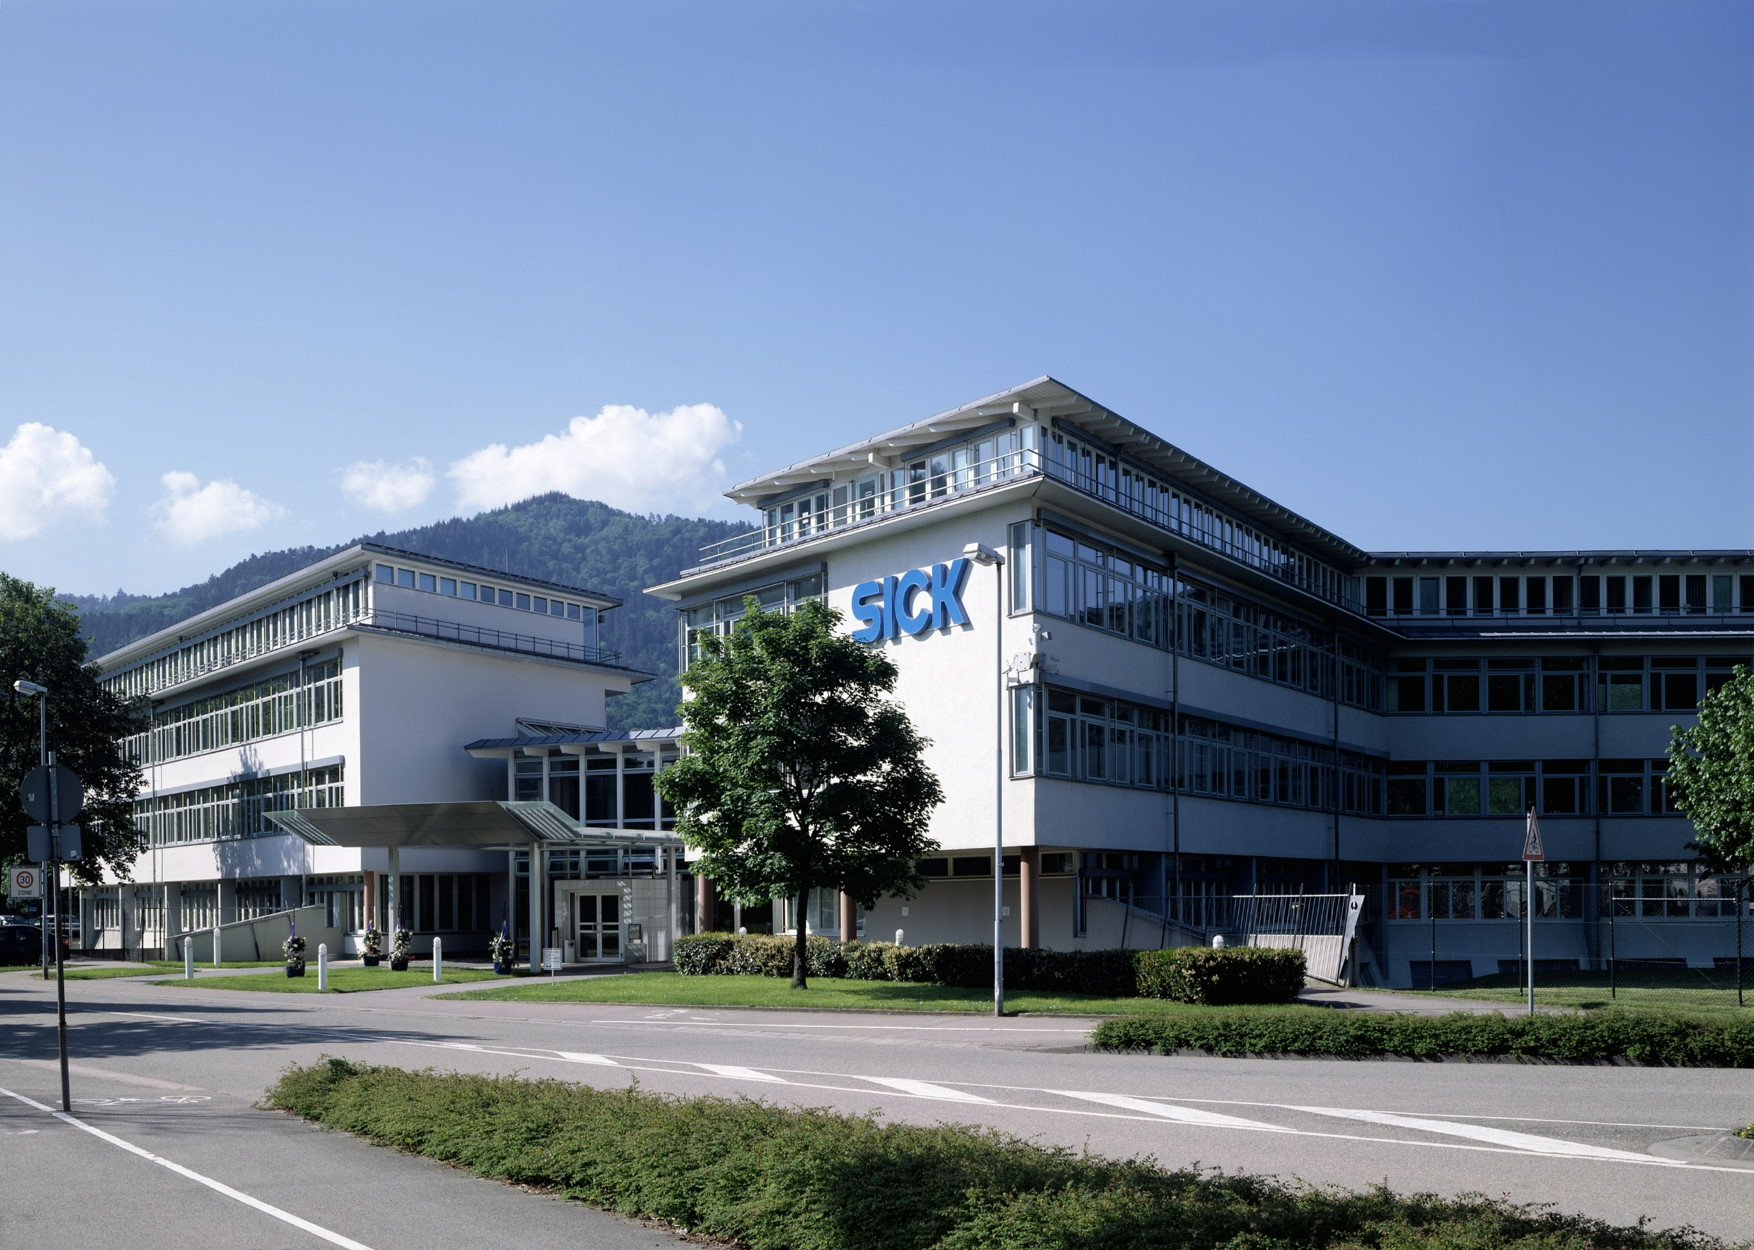
\includegraphics[width=(\textwidth/2)]{Bild/SICK_Headquarter.jpg}
    \caption{Hauptstandort der SICK AG\cite{.08.10.2016}}
    \label{fig:Hauptstandort der SICK AG}
\end{figure}
\fi
\subsection{Autonomous Perception}

Das Sick Business Cluster Autonomous Perception ist ein Teilbereich von Sick AG, der sich auf die Entwicklung von autonomen Wahrnehmungslösungen für den Einsatz in der Industrie konzentriert. Diese Lösungen ermöglichen es maschinellen Systemen, ihre Umgebung aktiv zu erkennen und auszuwerten, um dadurch sicherer und effizienter zu arbeiten.\\

Das Sick Business Cluster Autonomous Perception bietet eine Vielzahl von Produkten und Dienstleistungen, einschließlich 3D-Kameras, LIDAR-Sensoren und Software-Tools für die Datenanalyse. Diese Technologien ermöglichen es maschinellen Systemen, ihre Umgebung zu verstehen und Entscheidungen auf der Grundlage dieser Informationen zu treffen.\\

Einer der Hauptvorteile des Sick Business Cluster Autonomous Perception ist, dass es die Sicherheit und Effizienz in industriellen Prozessen erhöht. Durch die Fähigkeit, ihre Umgebung zu erkennen und auszuwerten, können maschinelle Systeme besser auf potenzielle Gefahren reagieren und vermeiden, dass sie Unfälle verursachen. Zusätzlich ermöglicht die Fähigkeit zur Datenanalyse, dass maschinelle Systeme ihre Leistung optimieren und ineffiziente Prozesse identifizieren und verbessern können.\\

\begin{figure}[htp]
    \centering
    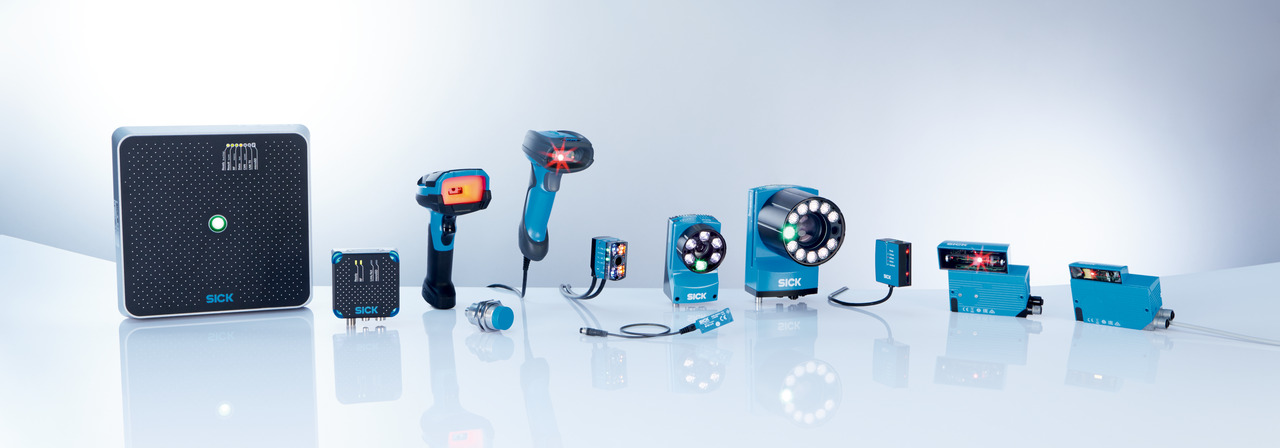
\includegraphics[width=(\textwidth)]{Bild/Identification solutions.jpg}
    \caption{Autonomous Perception\cite{.17.08.2021}}
    \label{fig:Autonomous Perception}
\end{figure}


\section{Problemstellung}
Die Problemstellung bei der Erstellung eines RFU-Client mit node-opcua liegt darin, eine effiziente und stabile Verbindung mit einem \ac{opcua}-Server herzustellen, um Daten auszutauschen und Anfragen zu stellen. 
Dies erfordert ein Verständnis der \ac{opcua}-Kommunikationsprotokolle und der Verwendung der node-opcua-Bibliothek, um die gewünschten Funktionalitäten zu implementieren. Mögliche Herausforderungen können darin bestehen, Fehlerbehandlungen zu implementieren, die Leistung zu optimieren und sicherzustellen, dass die Anwendung den Anforderungen des Benutzers entspricht.
\section{Ziel der Arbeit}
Das Ziel dieser Arbeit ist es, einen \ac{opcua}-Client in Node.js zu entwickeln, der in der Lage ist, sich mit dem Server des SICK RFUs zu verbinden und dabei das \ac{opcua}-Binary-Protokoll zu verwenden. \ac{opcua}-Binary ist plattformunabhängig und gilt als besonders sicher.\\

Um dieses Ziel zu erreichen, muss der Client zunächst die Verbindung zum Server anhand der IP-Adresse aufbauen können. Anschließend muss er in der Lage sein, verschiedene Methoden des Servers aufzurufen und diese fehlerfrei durchzuführen.\\

Zum Abschluss des Projekts soll eine grafische Benutzerschnittstelle entwickelt werden, die dem Benutzer ermöglicht, die Verbindung des Clients mit dem Server herzustellen und die Methoden des Servers zu nutzen, ohne den Quellcode ändern zu müssen.\\





\chapter{Grundlagen}
\section{Die OPC Foundation}
Die \ac{opc}-Technologie (OLE for Process Control) wurde entwickelt, um eine interoperable Kommunikation zwischen verschiedenen Plattformen unterschiedlicher Anbieter zu ermöglichen. Bis zum heutigen Zeitpunkt wird sie von über 17 Millionen Anwendungen genutzt \cite{OPCFoundation.15.06.2017}. Im Jahr 2016 wurde \ac{opc} und kann daher von jedem öffentlich auf Github gefunden werden, um die Adoption der Technologie zu erleichtern \cite{OPCFoundation.15.06.2017}.\\

\ac{opc} gilt als besonders sicher und zuverlässig und findet hauptsächlich Anwendung in der industriellen Automatisierung. Die Verantwortung für die Wartung und Entwicklung des Standards liegt bei der \ac{opc} Foundation. Der \ac{opc}-Standard definiert eine Vielzahl von Spezifikationen, die die Schnittstellen zwischen Clients und Servern, sowie zwischen Servern und Servern definieren. Dadurch wird es möglich, Ereignisse und Alarme zu überwachen, Zugriff auf Echtzeit- und historische Daten sowie auf andere Anwendungen zu erhalten.\\

Als \ac{opc} 1996 auf den Markt eingeführt wurde, war es auf speicherprogrammierbare Steuerungen (SPS) ausgelegt und konnte Lese- und Schreibbefehle ausführen. Dadurch war es möglich, Systeme und Produkte nahtlos über \ac{opc} zu kommunizieren \cite{OPCFoundation.15.06.2017}.

\subsection{OPC Unified Architecture}

\ac{opcua} ist ein Kommunikationsprotokoll für industrielle Automatisierungssysteme. Es wurde entwickelt, um eine sichere und zuverlässige Kommunikation zwischen verschiedenen Geräten und Systemen zu ermöglichen. Das Protokoll wurde 2006 eingeführt und hat sich seitdem zu einem weit verbreiteten Standard in der industriellen Automatisierungsbranche entwickelt.\\

\ac{opcua} ist plattformunabhängig und herstellerneutral konzipiert und ermöglicht die Kommunikation zwischen Geräten unterschiedlicher Hersteller. Es bietet eine gemeinsame Sprache für den Datenaustausch zwischen Geräten, was die Integration vereinfacht und das Risiko von Kompatibilitätsproblemen verringert. Darüber hinaus bietet \ac{opcua} eine Reihe erweiterter Funktionen, darunter Echtzeit-Datenzugriff, Ereignisüberwachung und Zugriff auf historische Daten.\\

Einer der Hauptvorteile von \ac{opcua} ist der Fokus auf Sicherheit. Das Protokoll enthält mehrere Sicherheitsfunktionen wie Verschlüsselung und digitale Signaturen, die vor unbefugtem Zugriff und Manipulation schützen. OPC UA verwendet auch ein mehrschichtiges Sicherheitsmodell, das dazu beiträgt, das Risiko von Sicherheitsverletzungen zu mindern.\\

\ac{opcua} ist außerdem skalierbar und flexibel konzipiert, wodurch es für den Einsatz in einer Vielzahl von industriellen Automatisierungsanwendungen geeignet ist. Das Protokoll kann sowohl in lokalen als auch in entfernten Anwendungen verwendet werden und unterstützt sowohl drahtgebundene als auch drahtlose Kommunikation.\\

Zusammenfassend lässt sich sagen, dass \ac{opcua} ein hochentwickeltes Kommunikationsprotokoll ist, das industriellen Automatisierungssystemen eine Reihe von Vorteilen bietet. Sein Fokus auf Sicherheit, Interoperabilität und Skalierbarkeit macht es zu einer idealen Lösung für eine Vielzahl von Anwendungen. Die weit verbreitete Übernahme von \ac{opcua} durch Hersteller und Anwender in der Industrieautomatisierungsbranche bestätigt seinen Wert und Nutzen.\\
\cite{Damm.2009}

\subsection{OPC Sicherheitsvorteile}

\ac{opcua} verfügt über ein großes und skalierbares Sicherheitskonzept, um eine hohe Zugriffsicherheit zu gewährleisten. Falls die Maßnahmen nicht ausreichen, können die Daten auf der Transport-Ebene mittels SSL verschlüsselt werden \cite{Team.06.03.2023}.\\

Um den Sicherheitsanforderungen der Anwendung gerecht zu werden, verfügt OPC UA über den Mechanismus der Endpunkte. Diese haben unterschiedliche Datenstrukturen und Sicherheitseigenschaften. Durch die Vereinheitlichung der Profile (Collaboration Models) können OPC UA-Clients den Inhalt der Daten interpretieren. \\

Für jede Funktion gibt es Profile wie den S95-Standard für die MES-Ankopplung\cite{Team.06.03.2023}. Um die Daten während der Übertragung zu sichern, werden 128- oder 256-Bit-Verschlüsselung, Nachrichtensignierung, Benutzerauthentifizierung und Paketsequenzierung verwendet.\\

OPC UA verwendet außerdem einen Zertifikataustausch, so dass sich jeder Client mittels eines Zertifikats authentifizieren muss. Dadurch wird sichergestellt, dass sich nur Clients mit dem Server verbinden, die auch die Erlaubnis haben \cite{Team.06.03.2023}.

\begin{figure}[htp]
    \centering
    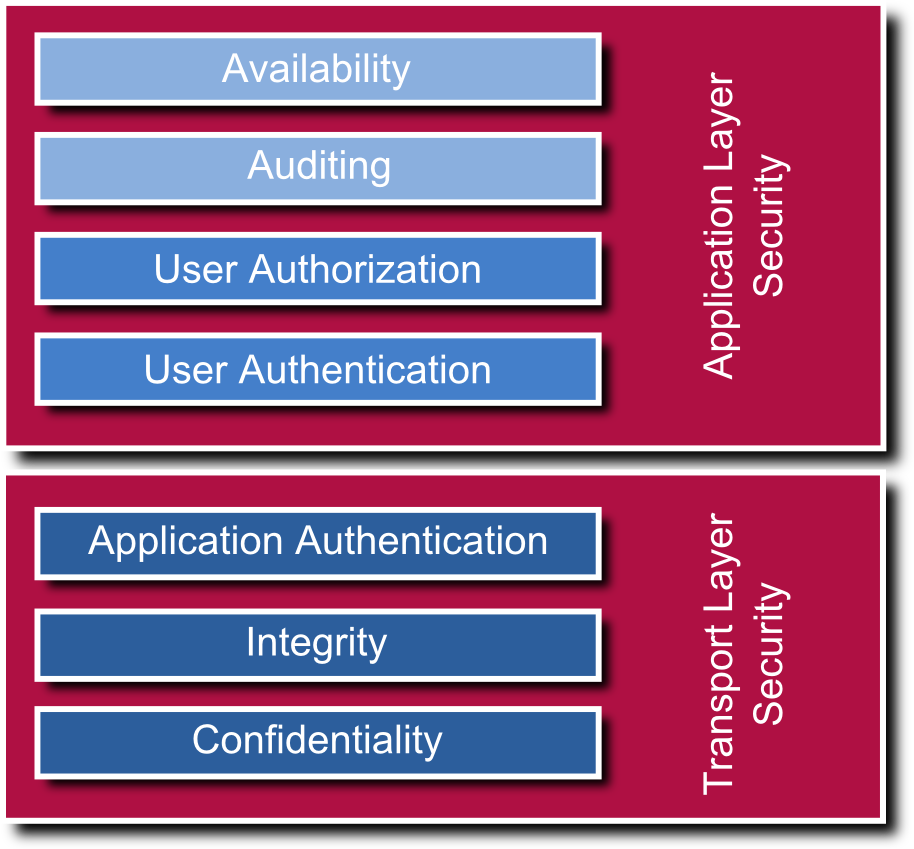
\includegraphics[width=(\textwidth/2)]{Bild/uasecurity.png}
    \caption{UA Sicherheit\cite{Team.06.03.2023}}
    \label{fig:UA Sicherheit}
\end{figure}

\section{Javascript}
JavaScript ist eine hochdynamische, objektorientierte Programmiersprache, die in den 1990er Jahren entwickelt wurde. Ursprünglich als Scriptsprache für Webbrowser konzipiert, wird sie heute in einer Vielzahl von Anwendungsbereichen eingesetzt, einschließlich Webentwicklung, mobilen Anwendungen, Desktop-Software und sogar im Internet der Dinge.\\

JavaScript ist eine interpretierte Sprache, was bedeutet, dass der Quellcode direkt ausgeführt wird, ohne dass er zuvor kompiliert werden muss. Dies ermöglicht es Entwicklern, schnell und einfach Prototypen zu erstellen und Feedback von Benutzern zu erhalten, ohne dass ein Kompilierungsprozess durchgeführt werden muss.\\

Ein wesentliches Merkmal von JavaScript ist seine Fähigkeit, asynchron zu arbeiten. Dies ermöglicht es der Sprache, gleichzeitig mehrere Aufgaben auszuführen, ohne dass die Benutzeroberfläche blockiert wird. Dies ist besonders wichtig bei der Entwicklung von Webanwendungen, da es Benutzern eine bessere Erfahrung ermöglicht, indem sie die Interaktivität und Reaktionszeit verbessert.\\

JavaScript unterstützt eine Vielzahl von Programmierparadigmen, einschließlich objektorientierter, funktionaler und prozeduraler Programmierung. Es bietet eine Fülle von Funktionen, die es Entwicklern ermöglichen, komplexe Anwendungen zu erstellen, einschließlich dynamischer Benutzeroberflächen, Datenbankanbindungen und Netzwerkanwendungen.\\

In Bezug auf die Syntax ähnelt JavaScript C-ähnlichen Sprachen, einschließlich C++ und Java. Es enthält jedoch auch einige einzigartige Funktionen, einschließlich hoher Dynamik und Unterstützung für reguläre Ausdrücke.\\

Zusammenfassend ist JavaScript eine vielseitige, leistungsstarke Programmiersprache, die für eine Vielzahl von Anwendungsbereichen verwendet werden kann. Ihre Fähigkeit, asynchron zu arbeiten, und ihre Unterstützung für mehrere Programmierparadigmen machen sie zu einer attraktiven Wahl für Entwickler.\\
 
\section{Node.js}
Node.js ist eine Open-Source, plattformübergreifende JavaScript-Laufzeitumgebung, mit der Entwickler skalierbare und leistungsstarke Anwendungen erstellen können. Es basiert auf der V8-Engine von Google, die JavaScript in Maschinencode kompiliert, um eine effiziente Ausführung zu ermöglichen. Node.js verwendet ein ereignisgesteuertes, nicht blockierendes E/A-Modell, das es gut geeignet macht, Anwendungen zu erstellen, die eine hohe Durchsatzrate und niedrige Latenzzeiten erfordern.\cite{.06.03.2023}\\

Einer der Schlüsselvorteile von Node.js ist seine Fähigkeit, große Anzahl von gleichzeitigen Verbindungen zu verarbeiten. Im Gegensatz zu herkömmlichen serverseitigen Technologien, die für jede eingehende Verbindung einen neuen Thread oder Prozess erstellen, verwendet Node.js einen einzigen Thread, um alle Verbindungen zu handhaben. Mit diesem Ansatz kann Node.js Tausende von gleichzeitigen Verbindungen verarbeiten, ohne übermäßige Systemressourcen zu verbrauchen.\cite{Node.js.27.02.2023b}\\

Node.js bietet auch ein umfangreiches Ökosystem von Bibliotheken und Modulen, die leicht installiert und in Anwendungen integriert werden können. Dies erleichtert es Entwicklern, komplexe Anwendungen schnell und effizient zu erstellen.\cite{Node.js.27.02.2023}\\

Ein weiterer Vorteil von Node.js ist seine Fähigkeit, auf verschiedenen Plattformen wie Linux, Windows und macOS ausgeführt werden zu können. Diese plattformübergreifende Kompatibilität macht es einfach, Code einmal zu schreiben und auf mehreren Plattformen bereitzustellen.\cite{Node.js.27.02.2023}\\

\section{Typescript}
TypeScript ist eine Programmiersprache, die eine Erweiterung von JavaScript darstellt. Sie bietet optional statisches Typing, was Entwicklern ermöglicht, Fehler vor der Laufzeit zu erkennen, was das Schreiben und die Pflege von komplexem Code erleichtern kann. TypeScript wurde von Microsoft entwickelt und ist heute eine Open-Source-Sprache, die in jedem JavaScript-Projekt verwendet werden kann. TypeScript erweitert JavaScript um Funktionen wie Schnittstellen, Klassen und Typannotationen.\cite{.01.03.2023b}\\

Einer der Vorteile von TypeScript besteht darin, dass es dazu beitragen kann, die Code-Qualität und Wartbarkeit zu verbessern. Durch die Verwendung von statischem Typing können Entwickler Fehler früh im Entwicklungsprozess erkennen, was zu leichter lesbarem Code führen kann. Darüber hinaus bietet TypeScript bessere Werkzeuge und Code-Intelligenz, was es einfacher macht, mit großen Code-Basen zu arbeiten und mit anderen Entwicklern zusammenzuarbeiten.\cite{.06.03.2023b}\\

TypeScript ist auch kompatibel mit beliebten JavaScript-Bibliotheken und Frameworks, was es einfach macht, in vorhandene Projekte zu integrieren. Es kann für Front-End-Entwicklung mit Frameworks wie Angular, React und Vue.js sowie für Back-End-Entwicklung mit Node.js verwendet werden.\cite{Udemy.06.03.2023}\\

Zusammenfassend ist TypeScript eine leistungsfähige Sprache, die dazu beitragen kann, die Code-Qualität und Wartbarkeit zu verbessern. Seine Kompatibilität mit beliebten JavaScript-Bibliotheken und Frameworks sowie seine umfangreichen Werkzeuge und Code-Intelligenz machen es zu einer beliebten Wahl unter Entwicklern. Entwickler können Ressourcen wie die offizielle TypeScript-Website, die TypeScript-Dokumentation und TypeScript-Tutorials von Udemy finden, um mit TypeScript zu beginnen.\cite{.01.03.2023}\\

\section{Der SICK RFU6 und seine Ensatzgebiete}

Der RFU ist eine intelligente Identifikationslösung von SICK AG und basiert auf der \ac{rfid}-Technologie, die für Radio Frequency Identification steht. Durch den Einsatz von Funkwellen ist es möglich, Objekte automatisch zu identifizieren. Ein \ac{rfid}-Transponder, der an dem Objekt angebracht ist, wird vom RFU erkannt und die darauf gespeicherten Daten ausgelesen. Es gibt drei verschiedene Arten von \ac{rfid}-Transpondern. Passive Transponder nutzen die Energie des elektromagnetischen Feldes des \ac{rfid}-Readers, um Daten zu senden und zu empfangen. Semi-passive und aktive Transponder haben zusätzlich eine Batterie, die eine höhere Reichweite ermöglicht und es ihnen ermöglicht, Daten wie Temperatur oder Feuchtigkeit zu erfassen und zu speichern.\cite{.07.03.2023}\\

Die Größe des SICK \ac{rfid}-Readers variiert und beeinflusst vor allem die Lese-Reichweite. Der RFU ist in der Lage, auch verschmutzte und verdeckte Objekte zu erkennen, da keine Sichtverbindung zum Transponder erforderlich ist. Die \ac{rfid}-Technologie gilt allgemein als sehr fehlerverzeihend und flexibel, da weder eine exakte Laserlinie noch eine bestimmte Schärfentiefe beachtet werden muss. Die Identifikation großer Objekte mit undefinierter Transponderposition ist durch hohe Leseabstände kein Problem. Die Datenübertragung ist verschlüsselt, was eine hohe Fälschungssicherheit und Datenschutz gewährleistet.\cite{.07.03.2023}\\

\ac{rfid}-Reader sind in der Industrie sehr vielseitig einsetzbar. Sie werden oft für die Werkstückidentifikation in der Prozessautomation oder für die Rückverfolgung von Transportbehältern in der Logistik eingesetzt. Sie eignen sich auch für die Überwachung des Warenein- und -ausgangs in der Logistik oder zur Identifikation von Zügen und Waggons im Schienenverkehr sowie zur elektronischen Mauterfassung.\cite{.07.03.2023}\\
\cite{.07.03.2023}

\begin{figure}[H]
    \centering
    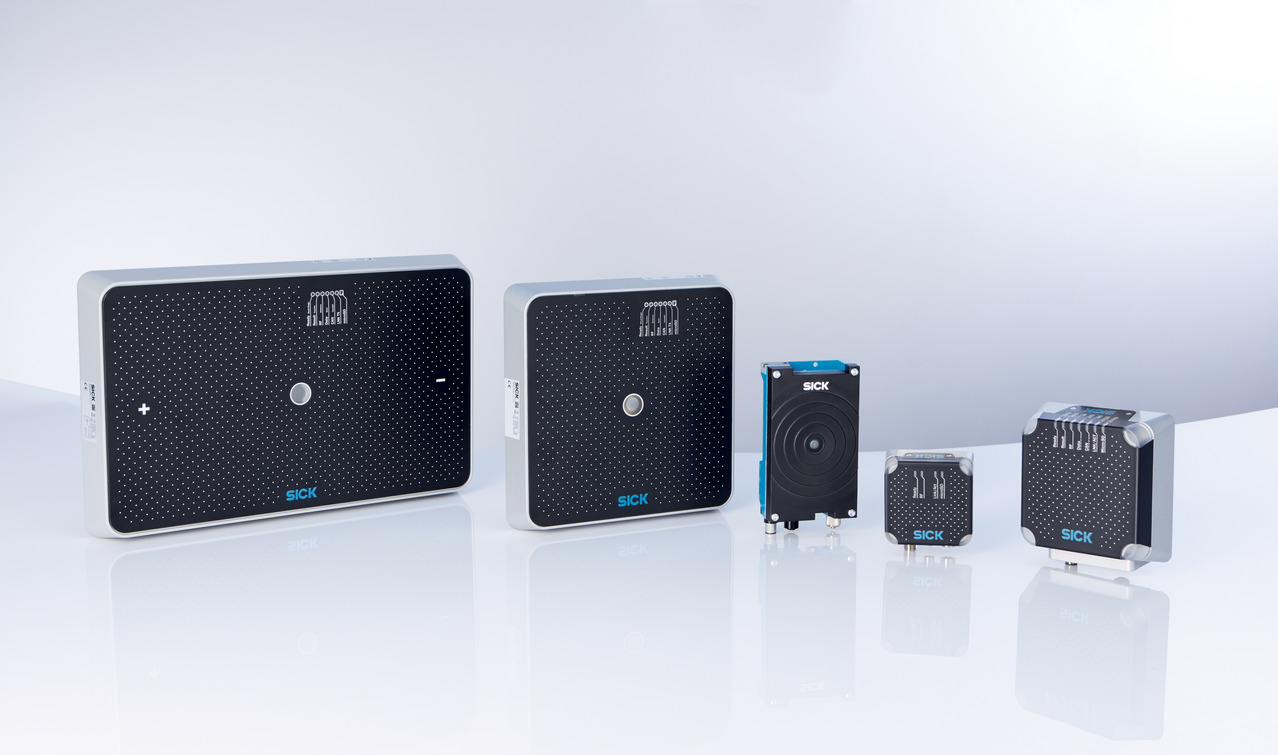
\includegraphics[width=(\textwidth/2)]{Bild/RFU.jpg}
    \caption{RFU\cite{.17.08.2021}}
    \label{fig:RFU}
\end{figure}


\section{UAExpert}
Der UaExpert ist ein OPC UA Testclient, der als universeller OPC UA Testclient entwickelt wurde und Funktionen wie DataAccess, Alarms \& Conditions, HistoricalAccess und den Aufruf von OPC UA Methoden unterstützt. Der Testclient wurde in C++ programmiert und ist plattformunabhängig. Die Benutzeroberfläche wurde mit der GUI-Bibliothek Qt erstellt und kann durch zusätzliche Plugins erweitert werden.\\

Das Basissystem des UaExpert umfasst grundlegende Funktionen wie Zertifikatsmechanismen, Discovery Service, Verbindungsherstellung, Browsing des Informationsmodells und das Lesen von Attributen und Referenzen von OPC UA Knoten. Die Projektansicht zeigt die OPC UA Server und die Adressraum-Ansicht stellt das Informationsmodell des OPC UA Servers in einer Baumstruktur dar. Die Ansichten der Dokument-Plugins befinden sich im Zentrum des Fensters, einschließlich der OPC UA DataAccess View, die Variablen beobachtet und Werte, Zeitstempel und den Status einzelner Knoten anzeigt. Weitere Ansichten können mit dem "Add Document" -Button hinzugefügt werden.\\
\section{Wireshark}
Wireshark ist ein Open-Source-Netzwerkprotokoll-Analyzer, der verwendet wird, um Netzwerkverkehr aufzufangen, zu analysieren und zu visualisieren. Mit Wireshark können Benutzer den gesamten Datenverkehr auf einem Netzwerk überwachen und analysieren, einschließlich der Informationen, die zwischen verschiedenen Geräten und Anwendungen ausgetauscht werden. Es ermöglicht Benutzern, den Datenverkehr in Echtzeit oder aus zuvor aufgezeichneten Daten zu analysieren und Probleme in der Netzwerkkommunikation zu identifizieren und zu beheben.










\chapter{Konzept}
Im Folgenden wird die Anwendung der in Kapitel 2 erläuterten Grundkonzepte beschrieben. Dabei wird zunächst auf den Entwurf der Software eingegangen, anschließend auf die prototypische Implementierung.\\

\section{Ausgangssituation}
In der Ausgangssituation wird der aktuelle Stand der Forschung im Bereich RFU-Client in Verbindung mit einem \ac{opcua}-Server und die Verbindung mit dem UAExpert untersucht. Es wird auch untersucht, was bisher mit Node \ac{opcua} erforscht wurde und welche \ac{opcua}-Clients bisher für den RFU verfügbar sind.

%aktueller Stand der Forschung
%welche verbindungen gibt es mit dem UAExpert? 
%Was wurde bisher mit node opcua gemacht?
%Welche Client gibt es bisher?
\subsection{Schnittstellen zum Server}
Auf dem RFU läuft ein \ac{opcua}-Server, der auf verschiedene Arten abgefragt wird. Einerseits gibt es verschiedene Clients, die in den Programmiersprachen Python, C\# oder C implementiert sind und alle mit dem Stack ihrer jeweiligen Programmiersprache arbeiten. Andererseits ist es auch möglich, den \ac{opcua}-Server mithilfe von UAExpert abzufragen und Daten zu empfangen.\\

Die Verbindung zum RFU wird über ein LAN-Kabel und einen USB-Internet-Adapter hergestellt. Der Internet-Adapter wird verwendet, da er frei konfiguriert werden kann. Die IP-Adresse des RFUs und des Internet-Adapters müssen im gleichen Subnetz liegen. Zunächst wird die IP-Adresse des RFUs konfiguriert. Diese kann über Sopas ET eingestellt werden. Danach wird die IP-Adresse des USB-Internet-Adapters konfiguriert.\\

Im UAExpert wird ein Server hinzugefügt. Unter \frqq Custom Discovery \flqq wird auf den \ac{opcua}-Server des RFUs über dessen zuvor konfigurierte IP-Adresse zugegriffen. In diesem Fall wird diese IP-Adresse genutzt: \frqq opc.tcp://192.168.136.2:4840 \flqq \\

\subsection{Die Struktur des Sensors}

Der UA-Experte ist in der Lage, die Objekte des Servers und die dazugehörigen Methoden mit Variablen des Servers auszulesen und grafisch darzustellen. Die Struktur des Sick RFU besteht aus vielen Knoten, von denen jeder aus verschiedenen Elementen besteht. Die Struktur des Sick RFU wird im Address Space Window dargestellt.\\

\begin{figure}[htp]
    \centering
    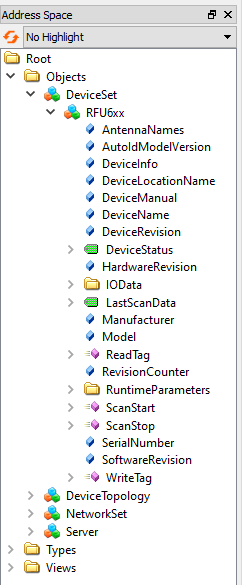
\includegraphics[width=(\textwidth/3)]{Bild/Address_Space.PNG}
    \caption{Address Space Window}
    \label{fig:Address Space Window}
\end{figure}

In der Abbildung \ref{fig:Address Space Window} wird die Struktur des Sensors mit seinen verschiedenen Elementen dargestellt, wobei jedes Element über einen eigenen Knoten verfügt. 
\frqq DeviceSet\flqq, \frqq RFU6xx\flqq, \frqq DeviceTopology\flqq, \frqq Networkset\flqq und \frqq Server\flqq sind Objekte, während die restlichen Elemente Methoden und Variablen darstellen. 
Im Rahmen dieses Projekts werden ausschließlich die in Lila markierten Methoden sowie der Knoten RFU6xx \frqq LastScanData\flqq benötigt. 
\frqq ReadTag\flqq, \frqq StartScan\flqq, \frqq WriteTag\flqq, \frqq StopScan\flqq und \frqq LastScanData\flqq sind die Methoden die in dem Node.js Client implementiert werden.

\subsection{Herstellung einer Verbindung}
Der \ac{opcua}-Client wird durch Node \ac{opcua} Bibliothek, die es ermöglicht, \ac{opcua}-Verbindungen aufzubauen. Die Bibliotheken erfordern die Angabe von entsprechenden Verbindungsdetails. Um den Client mit dem Server zu verbinden, wird die Bibliothek die Verbindungsdetails verwenden, die bei der Erstellung des Clients angegeben sind.
\begin{lstlisting}[style=JavaScript, caption={Node OPCUAClient Create}]
const options = {
    applicationName: "MyClient",
    connectionStrategy: connectionStrategy,
    securityMode: MessageSecurityMode.None,
    securityPolicy: SecurityPolicy.None,
    endpointMustExist: false,
};
const client = OPCUAClient.create(options);
const endpointUrl = "opc.tcp://192.168.136.2:4840";
async function main() {
    await client.connect(endpointUrl);
    console.log("connected !");
    const session = await client.createSession();
    console.log("session created !");
    await session.close();
    await client.disconnect();
    console.log("done !");
}
\end{lstlisting}

Der verwendete Port hängt von der Konfiguration des Servers und der verwendeten Verbindungsmethode ab. Standardmäßig wird in der Regel Port 4840 für \ac{opcua}-Verbindungen verwendet.

Eine Session ist eine Verbindung zwischen dem \ac{opcua}-Client und dem Server. Um eine Sitzung zu erstellen, muss der Client zunächst eine Verbindung zum Server herstellen und dann eine Anforderung für eine Sitzung senden. Die Node \ac{opcua}-Bibliotheken enthalten Funktionen zum Erstellen von Sitzungen.

Die Sitzung wird geschlossen, indem der \ac{opcua}-Client eine Anforderung zum Beenden der Sitzung sendet. Die Node \ac{opcua}-Bibliotheken verfügen über Funktionen zum Schließen von Sitzungen.

\subsection{RFU6xx Clients in anderen Programmiersprachen}

Es gibt bisher drei \ac{opcua}-RFU-Clients in verschiedenen Programmiersprachen. Die \ac{opcua}-RFU-Clients aus dem Hause Sick sind in den Programmiersprachen C\#, C und Python programmiert.\\

Die verschiedenen Clients greifen weitestgehend auf die gleichen Funktionen des \ac{opcua}-Servers des RFUs zu. \frqq ReadTag\flqq, \frqq StartScan\flqq, \frqq WriteTag\flqq, \frqq StopScan\flqq und \frqq LastScanData\flqq sind die Methoden, über die alle Clients verfügen.\\

Die Clients in den Programmiersprachen Python und C\# greifen auf die Funktionen des RFUs über eine Klasse zu, da sie es ermöglichen, objektorientiert zu programmieren. So können die Clients einfacher ausgelagert und spezifizierter verwendet werden. Der RFU-Client in der Programmiersprache C ist imperativ geschrieben.\\

Die RFU-Clients nutzen die Stacks ihrer Programmiersprache. Ein \ac{opcua}-Stack umfasst typischerweise verschiedene Module, einschließlich Transportebenen, Kodierungs- und Dekodierungsmodulen sowie Sicherheitsmodulen. Diese Module arbeiten zusammen, um eine vollständige Implementierung des \ac{opcua}-Protokolls bereitzustellen.\\

\ac{opcua}-Stacks können von Softwareentwicklern verwendet werden, um \ac{opcua}-fähige Anwendungen zu erstellen. Durch die Verwendung eines \ac{opcua}-Stacks können sich Entwickler auf ihre Anwendungslogik konzentrieren, ohne die Low-Level-Details des Protokolls implementieren zu müssen. Es gibt mehrere kommerzielle und Open-Source-\ac{opcua}-Stacks, die jeweils ihre eigenen Stärken und Schwächen haben.\\




\section{Softwareentwurf}


TypeScript ermöglicht sowohl imperatives als auch objektorientiertes Programmieren. Die Wahl hängt von der spezifischen Anforderung und Präferenz des Entwicklers ab.\\

Imperative Programmierung ist eine Programmiermethode, bei der das Programm als eine Folge von Anweisungen geschrieben wird, die in der Reihenfolge ausgeführt werden, in der sie geschrieben wurden. Sie ist nützlich, wenn Sie eine schnelle Lösung für ein bestimmtes Problem benötigen oder wenn Sie ein kleines Skript schreiben.\\

Objektorientierte Programmierung hingegen ist eine Programmiermethode, bei der das Programm als Zusammenstellung von Objekten und deren Interaktion geschrieben wird. Sie ist nützlich, wenn Sie eine komplexe Anwendung mit vielen Modulen und Komponenten schreiben. Mit objektorientierter Programmierung können Sie Ihre Codebasis besser strukturieren und wiederverwendbaren Code erstellen.\\

Für den spezifischen Einsatz des RFU-Clients wird er objektorientiert programmiert, damit er ausgelagert werden kann.\\

\subsection{Anforderungen}


Der RFU-Client soll leicht verständlich und leserlich sein.\\

Zunächst sollen Kommentare verwendet werden, um den Code zu dokumentieren und den Zweck der verschiedenen Abschnitte zu erklären. Dies kann dazu beitragen, dass der Code leichter zu verstehen ist, insbesondere wenn er komplexer wird.\\

Eine klare und konsistente Benennung von Variablen, Funktionen und Klassen, um den Code leichter lesbar und verständlich zu machen. Namen die den Zweck und die Funktion der Elemente klar ausdrücken.\\

Whitespace soll auch verwendet werden, um den Code leichter lesbar zu gestalten. Den Code so anordnen, dass er in Abschnitte oder Blöcke unterteilt ist, und Leerzeichen verwenden, um die verschiedenen Teile des Codes voneinander abzugrenzen.\\

Übermäßige Verschachtelung vermeiden, die den Code schwer lesbar machen kann. Stattdessen Funktionen oder Klassen, um den Code in kleinere Teile zu zerlegen, die zu verstehen sind.\\

\subsection{Systemumgebung}
Zudem wird in einer VM Programmiert. Programmiert wird in Nodepad++ und in vs code. Versioniert wird mit github.

\subsection{Programmdesgin}


\section{Vorgehensweise}
Wie wurde vorgegangen?
Woher wurden informationen gezogen?
Welche Beesonderheiten hatte TypeScript?


Der Python-Client, der als Vorlage dient, zeigt eine mögliche Implementierung eines Clients für ein Remote Field Unit 6xx (RFU6xx)-Gerät, das mit dem \ac{opcua}-Protokoll kommuniziert. Der Client ist in der Programmiersprache Python geschrieben und nutzt die Bibliothek "opcua" für die Kommunikation mit dem Gerät über das \ac{opcua}-Protokoll.\\

Die im Python-Client verwendeten Funktionen und Klassen können als Referenz für die Implementierung eines ähnlichen Clients in einer anderen Programmiersprache verwendet werden. Dabei können die verwendeten Konzepte wie asynchrone Programmierung, Verwendung von Namespace-Indizes, Anwendung von Strukturierungsmustern wie Funktionen und Klassen sowie die Verwendung von ExtensionObjects und Nodes für die Interaktion mit dem Gerät nützlich sein.\\

Es ist jedoch zu beachten, dass die tatsächliche Implementierung eines \ac{opcua}-Clients je nach Sprache und Bibliothek, die verwendet wird, unterschiedlich sein kann. Daher sollte der Python-Client als Beispiel und nicht als exakte Vorlage verstanden werden.\\







\chapter{Implementierung}
Nochmal die Forschungsfrage formulieren\\
Wie kann sich mit dem RFU6 über node opcua vebunden werden und auf dessen Methoden zugegriefen werden?


\section{Abfragen der Ids}
Um Methoden aufzurufen werden die jeweiligen NodeIds der verschiedenen Knoten benötiegt. 

OPC UA verwendet Namespaces, um eindeutige Kennungen über verschiedene Namensbehörden hinweg zu erstellen, die OPC UA-Informationmodelle definieren.\\

Die Attribute NodeId und BrowseName sind Kennungen eines Knotens. Ein Knoten im OPC UA-Adressraum wird eindeutig durch eine NodeId identifiziert. Im Gegensatz dazu kann der BrowseName nicht verwendet werden, um einen Knoten eindeutig zu identifizieren, da verschiedene Knoten denselben BrowseName haben können. Der BrowseName wird verwendet, um einen Pfad zwischen zwei Knoten zu erstellen oder eine Standard-Eigenschaft zu definieren.\\

Ein Namespace wird durch einen Namespace-URI identifiziert. Der URI ist der Bezeichner für ein OPC UA-Informationmodell, das von einer Arbeitsgruppe als Namensbehörde entwickelt wurde. Der URI für den Basis-OPC-UA-Namespace, der von der OPC-UA-Arbeitsgruppe definiert wurde, lautet \url{'http://opcfoundation.org/UA/'}.\\

Ein oder mehrere Instanz-Namespaces werden verwendet, um die serverspezifischen Instanzen von Standard- oder anbieterspezifischen Objekttypen bereitzustellen. Objektinstanzen sollten nicht mit Typknoten in einem Namespace gemischt werden, solange diese Typknoten in verschiedenen Servern wiederverwendet werden.\cite{.01.03.2021}\\

Sowohl die NodeId als auch der QualifiedName (DatenTyp für BrowseName) enthalten einen NamespaceIndex und eine Kennung. Der NamespaceIndex ist der Index in einer Namespace-Tabelle, die vom OPC UA-Server verwaltet wird. Die Namespace-Tabelle ist eine Eigenschaft, bei der der Wert ein Array von Zeichenfolgen ist. Jede Zeichenfolge ist ein Namespace-URI, der vom Server verwendet wird. Der Index in diesem Array ist der NamespaceIndex, der in NodeId und QualifiedName verwendet wird. Siehe auch OPC UA NodeId-Konzepte.\\

Um auf die Methoden des RFU6 zuzugreifen, werden die Namespace-Indizes der Node-IDs benötigt. Auch müssen die Ids für jeden Sitzung neue abgefragt werden da, sich die Ids verändern könnten.\\

Server dürfen den Namespace-Index für eine bestimmte Namespace-URI nicht ändern oder Einträge aus der Namespace-Tabelle löschen, solange eine aktive Sitzung besteht. So können Clients die Namespace-Tabelle für eine bestimmte Sitzung zwischenspeichern. Ein Server darf jedoch Namespace-Indizes ändern und Einträge aus der Namespace-Tabelle löschen, wenn kein Client verbunden ist oder wenn der Server neu gestartet wird. 
Aus diesem Grund sollte ein Client den Namespace-Index nicht speichern, ohne auch die Namespace-URI zu speichern, da eine Namespace-URI, die während einer Sitzung durch den Index \frqq  2 \flqq dargestellt wird, während der nächsten Sitzung durch den Index \frqq  5 \flqq dargestellt werden könnte. Daher sollte ein Client immer die Namespace-Tabelle des Servers lesen und die Namespace-Indizes aktualisieren, bevor er Dienste aufruft, bei denen NodeIds involviert sind, nachdem er eine Sitzung mit einem Server hergestellt hat.\\

Es gibt mehrere Möglichkeiten auf die NamespaceIndexe der NodeIds zuzugreifen.\\ 

Eine Möglichkeiten  ist die einen Addressraum zu erstellen und auf dessen Methode \frqq getNamespaceindex\flqq   auf die Id zuzugreifen.

Das Hauptziel des OPC UA-Adressraums ist es, eine standardisierte Möglichkeit für Server bereitzustellen, Objekte für Clients darzustellen. Das OPC UA-Objektmodell wurde entworfen, um dieses Ziel zu erreichen. Es definiert Objekte in Bezug auf Variablen und Methoden. Es ermöglicht auch die Darstellung von Beziehungen zu anderen Objekten.\cite{.11.04.2020}\\

\begin{lstlisting}[style=JavaScript, caption={Zugriff auf die Ids über den Addressraum}]
this.addressSpace = AddressSpace.create();
const namespace0 = this.addressSpace.getDefaultNamespace();

this.addressSpace.registerNamespace('http://opcfoundation.org/UA/AutoID/');
this.nsAutoID = this.addressSpace.getNamespaceIndex('http://opcfoundation.org/UA/AutoID/');
if (this.nsAutoID === -1) throw new Error(" cannot find AutoID namespace" );

this.addressSpace.registerNamespace(" http://opcfoundation.org/UA/DI/" );
this.nsOpcDI = this.addressSpace.getNamespaceIndex(" http://opcfoundation.org/UA/DI/" );

this.addressSpace.registerNamespace('http://www.sick.com/RFU6xx/');
this.nsRfu = this.addressSpace.getNamespaceIndex('http://www.sick.com/RFU6xx/');
\end{lstlisting}

In Zeile sechs wird eine Überprüfung auf minus eins durchgeführt. Wenn der Namespace zuvor nicht registriert ist, wird wird minus als Index zurückgegeben. Die Ids werde hier im Konstruktor abgefragt.\\

Die zweite Möglcihkeit ist es über die Session auf das Namespace Array zuzugreifen. Aus diesem Array werdem die NamespaceIndexe ausgelesen.\\

Der Index, den ein OPC UA-Server für eine Namespace-URI verwendet. Die Namespace-URI identifiziert die Namensautorität, die die Bezeichner von NodeIds definiert, z.B. die OPC Foundation, andere Standardisierungsgremien und Konsortien, das zugrunde liegende System oder den lokalen Server. Sie werden im sogenannten Namespace-Array (auch Namespace-Tabelle genannt) gespeichert. Namespace-Indizes sind numerische Werte, die zur Identifizierung von Namespaces zur Optimierung von Übertragung und Verarbeitung verwendet werden. Der Namespace-Index ist der Index der Namespace-URI im Namespace-Array.\\

\begin{lstlisting}[style=JavaScript, caption={Zugriff auf die Ids über die Session}]
async init(){		
    const nsArray = await this.session.readNamespaceArray();
    this.nsAutoId = this.session.getNamespaceIndex('http://opcfoundation.org/UA/AutoID/');
    this.nsOpcDI  = this.session.getNamespaceIndex(" http://opcfoundation.org/UA/DI/" );
    this.nsRfu    = this.session.getNamespaceIndex('http://www.sick.com/RFU6xx/');
}
\end{lstlisting}

Der Zugriff auf das Namespace-Array über die Session und damit auf die Methode \frqq readNamespaceArray()\flqq   hat den Nachteil, dass diese nicht im Konstruktor aufgerufen werden kann. Die Methode \frqq readNamespaceArray()\flqq   kann nicht im Konstruktor aufgerufen werden, da sie asynchron ist.\\

Asynchrone Funktionen können null oder mehrere await-Ausdrücke enthalten. Await-Ausdrücke bewirken, dass Promises-rückkehrende Funktionen sich so verhalten, als ob sie synchron wären, indem sie die Ausführung aussetzen, bis das zurückgegebene Promise erfüllt oder abgelehnt wird. Der aufgelöste Wert des Promise wird als Rückgabewert des await-Ausdrucks behandelt. Die Verwendung von async und await ermöglicht die Verwendung von gewöhnlichen try/catch-Blöcken um asynchronen Code.\\

Somit ist die Funktion \frqq async init()\flqq   erforderlich, da es nur innerhalb von async-Funktionen möglich ist, \frqq await\flqq   zu verwenden.\\

Der Zugriff auf NodeIds über den AddressSpace hat den Nachteil, dass er zwar positive Werte liefert, aber nicht mit den tatsächlichen NodeIds übereinstimmt, die mit dem UAExpert ausgelesen werden können.

Da durch fehlerhafte IDs das Aufrufen der Methoden des RFU6 nicht möglich ist, wird die Session verwendet, um auf die NodeIds zuzugreifen

\section{StartScan CallMethod}

Vergleiche die Online vorlage mit der aktuellen Version

Was soll die Methode StartScan machen?

Wie seiht die Methode in Python aus?

Die StartScan-Methode startet den Scan des RFU6. Der RFU6 ist in der Lage, RFID-Tags zu lesen. Zur Entwicklung der StartScan-Methode in einem OPC UA-Node kann die bereits implementierte StartScan-Methode des Python-Clients als Vorbild genommen werden.

\begin{lstlisting}[style=Python, caption={StartScan Python},label={StartScanPython}]
async def StartScan(self,duration : float, cycle: int, dataAvailable : bool):
    db = struct.pack("IdI?",0,duration,cycle,dataAvailable)
    eo = ExtensionObject(TypeId=ua.NodeId.from_string(f"ns={self.nsAutoID};i=3010"), Body=db)
    return await self.rfu6xxNode.call_method(f"{self.nsAutoID}:ScanStart", eo) 
\end{lstlisting}

Die Funktion \dq StartScan\dq  definiert eine Methode, die asynchron ausgeführt wird und erwartet die Angabe von drei Parametern. Der erste Parameter ist \dq duration\dq , eine Gleitkommazahl, die die Dauer des Scans in Sekunden angibt. Der zweite Parameter ist \dq cycle\dq , eine ganze Zahl, die die Anzahl der Zyklen angibt, die während des Scans durchgeführt werden sollen. Der dritte Parameter ist \dq dataAvailable\dq , ein boolescher Wert, der angibt, ob während des Scans Daten verfügbar sein werden oder nicht.\\

Die Funktion konvertiert dann diese Parameter in einen Byte-String und erstellt damit ein \dq ExtensionObject\dq . Das ExtensionObject wird mit der NodeId des Methodenaufrufs \dq ScanStart\dq  und dem Namensraum (ns) des Objekts erstellt, das diese Methode bereitstellt. Das NodeId-Objekt wird durch Aufrufen der \dq from\_string\dq  -Methode mit einem String, der die NodeId im Format $ns=<namespace-Id>;i=<identifier>$ darstellt, erstellt.\\

Schließlich wird die Methode \dq ScanStart\dq  mit dem erstellten ExtensionObject als Parameter aufgerufen, indem die Methode \dq call\_method\dq  des Nodes \dq rfu6xxNode\dq  verwendet wird. Der Rückgabewert der Methode \dq ScanStart\dq  wird zurückgegeben, nachdem er mit dem Schlüsselwort \dq await\dq  auf seine Beendigung gewartet hat.\\

Insgesamt handelt es sich bei dieser Funktion um eine Methode, die einen Scan mit den angegebenen Parametern startet und auf die Beendigung des Scans wartet, bevor sie den Rückgabewert zurückgibt.\\

Was konnte man über Wireshark herausfinden?

Es ist möglich die StartScan Methode über den UAExpert auszuführen. Die Kommunikation zwischen des Servers der auf dem RFU6 läuft und dem UAExpert kann mit Wireshark überwacht werden. Den Aufruf der hier zu sehen ist soll reproduziert werden.


\begin{figure}[H]
    \centering
    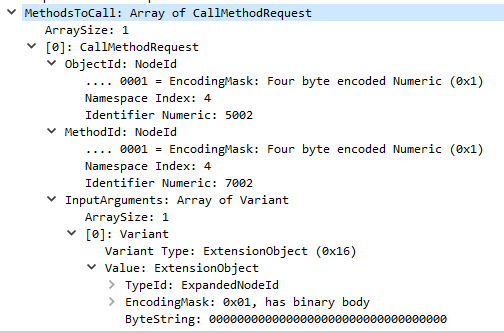
\includegraphics[width=(\textwidth/2)]{Bild/StartScabWireshark.PNG}
    \caption{StartScan über Wireshark}
    \label{fig:StartScanueberWireshark}
\end{figure}

Der OpcUa-Service ist ein \dq Encodeable Object\dq  mit dem TypeId \dq ExpandedNodeId\dq . Es wird eine \dq CallRequest\dq  ausgeführt, die einen \dq RequestHeader\dq  und eine \dq MethodToCall\dq -Liste enthält. Die Liste hat eine Größe von 1 und enthält einen \dq CallMethodRequest\dq . Dieser hat eine \dq ObjectId\dq  und eine \dq MethodId\dq , die jeweils durch eine \dq NodeId\dq  dargestellt werden.\\

Der \dq CallMethodRequest\dq  enthält auch eine \dq InputArguments\dq -Liste mit einer Größe von 1, die einen \dq Variant\dq  enthält. Dieser hat den Variant-Typ \dq ExtensionObject\dq  und einen \dq Value\dq , der wiederum ein \dq ExtensionObject\dq  ist. Dieses hat eine TypeId und einen ByteString mit einer Länge von 40 Bytes, der alle Nullen enthält.\\

Wie kann man die Methode aufrufen?

Ein Methodenaufruf ermöglicht es, Eingabe- und Ausgabeargumente an/von einer Methode zu übergeben. Diese Argumente werden durch Eigenschaften der Methode definiert.\\

Der Aufruf benötigt die NodeId der jeweiligen Methode. Die Node Ids können aus dem UAExpert oder aus dem Wireshark gelesen werden.
\begin{lstlisting}[style=JavaScript, caption={Methodenaufruf StartScan}]
const methodToCall: CallMethodRequestLike = {
    methodId: (`ns=${this.nsRfu};i=7002`),
    objectId: (`ns=${this.nsRfu};i=5002`),
    inputArguments: [
        {
        dataType: DataType.ExtensionObject,
        value: scanSettingsObj
        }
    ]
};

// Call method, passing ScanSettings as input argument
    await this.session.call(methodToCall,(err,results) => {
        if (err) {
            console.log(err);
        } else {
            console.log(results);
        }
    });
\end{lstlisting}

Der Code verwendet die OPC UA-Bibliothek und ruft eine Methode auf einem Remote-Server auf.\\

Der Code definiert zuerst ein Objekt namens \dq methodToCall\dq  mit den Eigenschaften \dq methodId\dq , \dq objectId\dq  und \dq inputArguments\dq . \dq methodId\dq  und \dq objectId\dq  definieren die OPC UA-Methoden-ID und Objekt-ID, die aufgerufen werden sollen. \dq inputArguments\dq  definiert die Eingabeargumente, die an die aufgerufene Methode übergeben werden sollen.\\

Dann wird die Methode mit \dq session.call\dq  aufgerufen und die Eingabeargumente werden übergeben. Das Ergebnis des Methodenaufrufs wird in einer Rückruffunktion verarbeitet, wobei eventuelle Fehler in der Konsole ausgegeben werden und das Ergebnis des Methodenaufrufs angezeigt wird.

\subsection*{Konstruieren eines Extensionobject}

Das ExtensionObject ist das Input-Argument für die StartScan-Methode. Es enthält die gleichen Parameter wie diejenigen, die auch in UAExpert eingegeben werden müssen, um den Scan zu starten. Im Python-Code \ref{StartScanPython} sind diese Parameter enthalten.\\

Was ist ein ExtensionObject?

Ein ExtensionObject ist ein Behälter für strukturierte Datentypen, die nicht als einer der anderen eingebauten Datentypen codiert werden können. Das ExtensionObject enthält einen komplexen Wert, der als Sequenz von Bytes oder als XML-Element serialisiert ist. Es enthält auch einen Identifier, der angibt, welche Daten es enthält und wie sie codiert sind.\\

Strukturierte Datentypen werden im Server-Adressraum als Unterarten des Strukturdatentyps dargestellt. Die verfügbaren Datenkodierungen für jeden Strukturierten Datentyp werden als DataTypeEncoding-Objekt im Server AddressSpace dargestellt. Die NodeId für das DataTypeEncoding-Objekt ist die Kennung, die im ExtensionObject gespeichert ist.\\

Es werden namensraumqualifizierte numerische NodeIds für alle definierten DataTypeEncoding-Objekte verwenden. Dies minimiert den Overhead, der durch das Verpacken von strukturierten Datentypwerten in ein ExtensionObject eingeführt wird.\\

Die OPCUA-Bibliothek enthält einen Test, der auch die \dq ScanSettings\dq  in ein \dq ExtensionObject\dq  kodiert. Die Eingaben, die zur Erstellung des \dq ExtensionObject\dq  verwendet werden, sind dieselben wie diejenigen, die in UA Expert eingegeben werden müssen, um den Scan zu starten.\\

\begin{lstlisting}[style=JavaScript, caption={ExtensionObject ScanSettings Test}]
enum LocationTypeEnumeration {
    NMEA = 0, // An NMEA string representing a coordinate as defined in 9.1.2.
    LOCAL = 2, // A local coordinate as defined in 9.3.4
    WGS84 = 4, // A lat / lon / alt coordinate as defined in 9.3.16
    NAME = 5 // A name for a location as defined in 9.1.1
}
interface ScanSettings extends ExtensionObject {
    duration: number;
    cycles: number;
    dataAvailable: boolean;
    locationType?: LocationTypeEnumeration;
}
const scanSettingsDataTypeNode = addressSpace.findDataType("ScanSettings", nsAutoId)!;

const settings = addressSpace.constructExtensionObject(scanSettingsDataTypeNode, {}) as ScanSettings;
\end{lstlisting}

Der Code definiert eine Enumeration namens \dq LocationTypeEnumeration\dq , die verschiedene Arten von Ortsangaben für einen Scan darstellt, einschließlich Koordinaten in verschiedenen Formaten und einem Ortsnamen.\\

Dann wird eine Schnittstelle namens \dq ScanSettings\dq  erstellt, die das \dq ExtensionObject\dq  erweitert. Diese Schnittstelle enthält einige Eigenschaften wie \dq duration\dq  (Dauer), \dq cycles\dq  (Zyklen), \dq dataAvailable\dq  (Daten verfügbar) und optional \dq locationType\dq  (Ortsangabe-Typ).\\

Das \dq ExtensionObject\dq  ist ein Container für strukturierte Datentypen, die nicht als einer der anderen eingebauten Datentypen kodiert werden können. Der Code verwendet die \dq constructExtensionObject\dq -Methode, um ein \dq ExtensionObject\dq  vom Typ \dq ScanSettings\dq  zu erstellen.\\

Beim Versuch, den Code auszuführen, treten Fehler auf, da es nicht möglich ist, die NodeId für das \dq ExtensionObject\dq  mit der Methode \dq findDataType\dq  zu finden.\\

Es ist jedoch möglich, die NodeId des jeweiligen UAExpert auszulesen oder sie im Wireshark zu suchen und diese dann hardcoded in den Code einzutragen.\\

\begin{lstlisting}[style=JavaScript, caption={ScanSettingsObj}]
const scanSettingsParams = {
    duration : aduration,
    cycles : acycles,
    dataAvailable : adataAvailable,
    locationType: 0
}
// NodeID for InputArguments struct type (inherits from ScanSettings)
const nodeID = new NodeId(NodeIdType.NUMERIC, 3010, 3);

// Create ExtensionObject for InputArguments
const scanSettingsObj = await this.session.constructExtensionObject(nodeID, scanSettingsParams)
\end{lstlisting}

Zunächst wird eine NodeId-Objekt erstellt, das die numerische ID des Typs der Struktur InputArguments enthält, die von der ScanSettings-Struktur erbt.\\

Das NodeId-Objekt wird mit Hilfe des new Schlüsselwortes und des NodeIdType.NUMERIC Enumerators erstellt. Der erste Parameter gibt den Typ der NodeID an und der zweite und dritte Parameter geben die numerischen Werte der NodeID an.\\

Dann wird die constructExtensionObject-Methode der Session-Klasse aufgerufen, um das ExtensionObject-Objekt zu erstellen. Diese Methode nimmt zwei Parameter entgegen, nämlich die NodeId und das scanSettingsParams-Objekt, das die Einstellungen des Scans enthält.\\

Das Schlüsselwort await wird verwendet, um die asynchrone Ausführung des Codes zu ermöglichen und sicherzustellen, dass das scanSettingsObj-Objekt vollständig erstellt wird, bevor es verwendet wird. Das resultierende Objekt ist das ExtensionObject, das die Einstellungen des Scans im System enthält.\\

Das erstellte ExtensionObject kann als inputArgument in den MethodenRequest aufgenommen werden und den Scan zustarten.

\section{LastScanData ReadMethode}
Was soll die Methode zurückgegeben?

Die Methode gibt die Daten des letzten Scans zurück. Diese beinhalten die TagId eines möglichen RFID-Tags, der vom RFID-Scanner gescannt wird. Um auf die Daten zuzugreifen, muss zuvor die StartScan-Methode aufgerufen werden und es müssen Daten empfangen werden.\\

Was ist ein Session read?

Um auf die Knoten LastScanData zuzugreifen, ist keine Methode mit einem MethodRequest erforderlich, sondern eine Read-Methode.\\

Dieser Service wird verwendet, um ein oder mehrere Attribute von einem oder mehreren Knoten zu lesen. Bei konstruierten Attributwerten, deren Elemente indexiert sind, z.B. ein Array, ermöglicht dieser Service den Clients das Lesen des gesamten Satzes indexierter Werte als Composite, das Lesen einzelner Elemente oder das Lesen von Bereichen von Elementen des Composite.\\

Der Parameter \dq maxAge \dq wird verwendet, um den Server anzuweisen, den Wert aus der zugrunde liegenden Datenquelle, wie z.B. einem Gerät, abzurufen, wenn dessen Kopie der Daten älter ist als das, was der "maxAge" angibt. Wenn der Server das angeforderte maximale Alter nicht erfüllen kann, gibt er seinen "besten Versuchswert" zurück, anstatt die Anfrage abzulehnen. MaxAge wird beim erstellen des Client festgelegt.\\

\begin{lstlisting}[style=JavaScript, caption={ScanSettingsObj}]
const nodeToRead = {
    nodeId:      `ns=${this.nsRfuId};i=6023`,
    attributeId: AttributeIds.Value
};
const lastScanData = await this.session.read(nodeToRead);
return lastScanData.value.value;
\end{lstlisting}
Der Code definiert zunächst eine Konstante namens \dq nodeToRead\dq , die ein Objekt-Literal enthält. Dieses Objekt hat zwei Eigenschaften: \dq nodeId\dq  und \dq attributeId\dq . Die \dq nodeId\dq  Eigenschaft enthält eine Zeichenkette, die die Node-ID im OPC-UA-Server angibt, von der Daten gelesen werden sollen. Die \dq attributeId\dq  Eigenschaft gibt an, welches Attribut des Knotens (Node) gelesen werden soll. In diesem Fall soll das Attribut \dq Value\dq  gelesen werden, was bedeutet, dass der tatsächliche Wert der Node zurückgegeben wird.\\

Anschließend wird eine weitere Konstante namens \dq lastScanData\dq  definiert, die auf das Ergebnis einer asynchronen Operation wartet. Diese asynchrone Operation wird mit \dq await\dq  und \dq this.session.read(nodeToRead)\dq  ausgeführt, wobei \dq this.session\dq  eine Referenz auf eine Verbindungssitzung zum OPC-UA-Server ist. Der Befehl \dq read\dq  liest die Daten von der angegebenen Node-ID im Server.\\

Schließlich wird der Wert der Eigenschaft \dq value\dq  im Objekt \dq lastScanData\dq  zurückgegeben, der den tatsächlichen Wert der gelesenen Node enthält. Die Node wurde aus einer Aufnahme von Wireshark gelesen als mit dem UaExpert LastScandata aufgerufen wird.

\section{ReadTag CallMethode}

Die ReadTag-Methode wird verwendet, um die Daten des Tags mit der entsprechenden ID auszulesen.

Auf dem RFID Tag können ByteString gespeichert werden. Die mit der Write Methode ausgelesen werden.

Wie das Inputargument aufgebaut wird, erdeutet sich aus dem UAExpert und aus dem Wireshark Aufnahme des UaExpert, wenn dieser die ReadTag Methode aufruft. 

\begin{figure}[H]
    \centering
    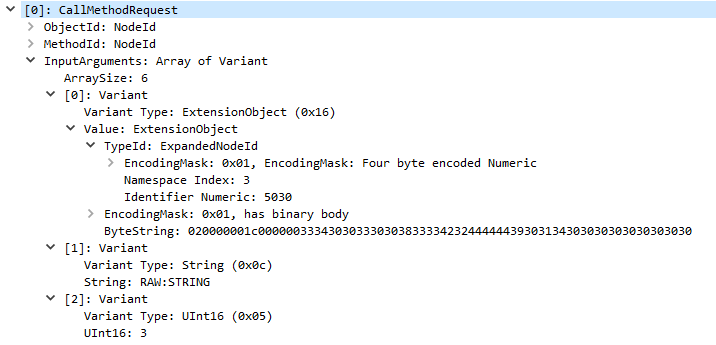
\includegraphics[width=(\textwidth/2)]{Bild/WriteTagWireshark.PNG}
    \caption{StartScan über Wireshark}
    \label{fig:WriteueberWireshark}
\end{figure}

\begin{lstlisting}[style=JavaScript, caption={ReadTag Methode}]
async ReadTag(tagId : string, codetype : string, region : number, offset : number, length : number){

    const identiferParams = {
        string: tagId	
    }

    const identifierId = new NodeId (NodeIdType.NUMERIC, 3020, 3);
    const identifierObj = await this.session!.constructExtensionObject(identifierId, identiferParams);
    
    const methodToCall : CallMethodRequestLike = {
        methodId : (`ns=${this.nsRfuId};i=7004`),
        objectId : (`ns=${this.nsRfuId};i=5002`),
        inputArguments : [{
            dataType : DataType.ExtensionObject,
            value : identifierObj
        },
        {
            dataType : DataType.String,
            value : codetype
        },
        {
            dataType : DataType.UInt16,
            value : region
        },
        {
            dataType : DataType.UInt32,
            value : offset
        },
        {
            dataType : DataType.UInt32,
            value : length
        },
        {
            dataType : DataType.String,
            value : ""
        }
        ]
    };
    this.session!.call(methodToCall,(err,results) => {
            if (err) {
                console.log(err);
            } else {
                console.log("ReadTag Result: ",results);
            }
        });
}
\end{lstlisting}

Dieser Code definiert eine asynchrone Funktion ReadTag, die fünf Argumente erwartet: tagId (ein String), codetype (ein String), region (eine Zahl), offset (eine Zahl) und length (eine Zahl). Die Funktion ruft eine Methode in einem OPC UA-Server auf, um den Wert eines Tags auszulesen.\\

In der Funktion wird zuerst ein Objekt identifierParams erstellt, das einen Parameter string enthält, der den Wert von tagId enthält. Dann wird ein neues NodeId-Objekt erstellt, das die numerische ID 3020 und den Typ 3 enthält. Diese NodeId-Instanz wird verwendet, um ein Extension-Objekt zu erstellen, das das identifierParams-Objekt als Parameter enthält. Das Ergebnis wird in der Variable identifierObj gespeichert.\\

Dann wird ein methodToCall-Objekt erstellt, das die Methoden-ID und Objekt-ID für den OPC UA-Server enthält. Die Eingabe-Argumente für die aufzurufende Methode werden ebenfalls in diesem Objekt definiert. Das identifierObj-Objekt wird als Extension-Objekt für das erste Argument verwendet, während die restlichen Argumente vom Typ DataType.String, DataType.UInt16, DataType.UInt32 und DataType.String sind.\\

Schließlich wird die call-Methode der session-Instanz aufgerufen, um die Methode auf dem OPC UA-Server auszuführen. Wenn ein Fehler auftritt, wird er in der Konsole ausgegeben. Andernfalls wird das Ergebnis der Methode in der Konsole ausgegeben.\\

Es ist zu beachten, dass die call-Methode asynchron ist und ein Callback-Funktion als zweites Argument erwartet, die aufgerufen wird, wenn die Methode auf dem Server ausgeführt wurde und ein Ergebnis zurückgegeben wurde. In diesem Fall wird der Callback verwendet, um das Ergebnis der Methode auszugeben.\\



\section{EventRegistration}
%Was soll die methode machen?

Die Methode registriert das Event RfidScanResult und gibt dieses in der Connsole aus.

Ein OPCUA Event zu registriert und zu abonieren ist wie Datenänderungen, aber anstatt einen Datenänderungsfilter zu verwenden wird ein Eventfilter verwendet.\\

%Was ist ein Events?

Events repräsentieren spezifische Ereignisse. Event-Benachrichtigungen melden das Auftreten eines Events. Objekte und Ansichten können genutzt werden, um sich für Events anzumelden. Das EventNotifier-Attribut dieser Knoten identifiziert, ob der Knoten das Abonnieren von Events erlaubt. Clients melden sich bei solchen Knoten an, um Benachrichtigungen über das Auftreten von Events zu erhalten.\\

Event-Abonnements verwenden Monitoring- und Abonnement-Dienste, um sich für die Event-Benachrichtigungen eines Knotens anzumelden.\\

Jeder OPC UA-Server, der Eventing unterstützt, muss mindestens einen Knoten als EventNotifier bereitstellen. Das Serverobjekt wird hierfür verwendet. Events, die vom Server generiert werden, stehen über dieses Serverobjekt zur Verfügung.\\

%Was ist ein Eventfilter?

Der EventFilter ermöglicht die Filterung und Auswahl von Event-Abonnements.
Wenn eine Event-Benachrichtigung dem Filter entspricht, wird sie an den Client gesendet. Der Event-Filter gibt an, welche Felder in der Event-Benachrichtigung
enthalten sein sollen und welche Event-Typen unterstützt werden. Der SimpleAttributeOperand Struktur wird verwendet, um die Event-Attribute auszuwählen, die zurückgegeben werden sollen.  Der EventFilter prüft auch auf strukturelle Fehler beim Erstellen oder Aktualisieren des
Filters.\\

%Wie ist das Vorgehen?

Es ist möglich die EventRegistration Methode über den UAExpert auszuführen. Bei der beobachtung mit Wireshark muss beachtet werden welche Paket relevant sind für die Anforderung an die Methode.

%Wie wird es im UAExpert gemacht?

%Was sagt Wireshark?

Die relevantesten Pakete sind die Erstellung einer Subscription und die Erstellung eines MonitoringItem.

%Was ist eine Subscription?

Eine Subscription wird dazu genutzt Nachrichten oder Benachrichtigung an
den Client zusenden. Subscriptions haben MonitoredItem die Benachrichtigungen generieren, die an den Client gesendet werden. Die Subscriptiom haben auch eine Veröentlichungsrate und eine Keep-alive -Zähler, der angibt,
wie viele Zyklen ohne Benachrichtigung es gegeben hat. Wenn der maximale
keep-alive-Zähler errechtj ist, wird eine Nachricht gesendet, um den Client
darüber zu informieren, dass die Subscription noch aktiv ist.\\
Nach der Erstellung der Subscription startet der Server den Veröentlichungstimer und startet ihn neu, wenn er abläuft. Wenn der Timer abläuft,
ohne dass vom Client eine Subscription-Service-Request empfangen wurde
und die Anzahl der Subscriptionlebensdauer abgelaufen ist, geht die Subscription davon aus, dass der Client nicht mehr vorhanden ist und wird beendet.\\

%Keep alive Count hat er was damit zu tun wann die Subcription geschlossen wird?
Wenn \dq keep-alive \dq den Wert erreicht, der für die Lebensdauer einer Subscription basierend auf dem MaxKeepAliveCount-Parameter im CreateSubscriptionService berechnet wird, wird die Subscription geschlossen.
Das Attribut gibt die Priorität des Abonnements an. Wenn mehrere
Abonnements Benachrichtigungen senden müssen, wird der Server die Veröentlichungsanfrage an das Abonnement mit der höchsten Priorität weiterleiten. Wenn die Keep-Alive-Zeit abläuft, hat das Abonnement Vorrang, um
das Ablaufen zu verhindern. Wenn ein Client keine besonderen Prioritätseinstellungen benötigt, sollte der Wert auf Null gesetzt werden.\\

%Was ist die CreateSubscription?
\begin{lstlisting}[style=JavaScript, caption={SubscriptionForEventRegistration}]
async SubscriptionForEventRegistration(){
    // step 5: install a subscription and install a monitored item for 10 seconds
    const subscription = ClientSubscription.create(this.session!, {
        requestedPublishingInterval: 500,
        requestedLifetimeCount: 2400,
        requestedMaxKeepAliveCount: 10,
        maxNotificationsPerPublish: 65535,
        publishingEnabled: true,
        priority: 0                   //the priority of a subscription, determining the order in which Publish requests are dequeued and processed by the server
    });

    subscription
        .on("started", function () {
        console.log(
            "subscription started for 2 seconds - subscriptionId=",
            subscription.subscriptionId
        );
        })
        .on("keepalive", function () {
        console.log("keepalive");
        })
        .on("terminated", function () {
        console.log("terminated");
        });
    return subscription;
}
\end{lstlisting}

Der Code implementiert eine asynchrone Funktion namens "SubscriptionForEventRegistration", die eine Subscription erstellt, um überwachte Elemente (monitored items) zu empfangen.\\

Es wird eine Subscription mit bestimmten Einstellungen erstellt, einschließlich des gewünschten Veröffentlichungsintervalls, der Anzahl der erwarteten Lebensdauerereignisse, der maximalen Anzahl von Keepalive-Ereignissen, die empfangen werden sollen, der maximalen Anzahl von Benachrichtigungen, die pro Veröffentlichung empfangen werden sollen, und der Priorität der Subscription.\\

Das "subscription" Objekt wird durch Aufruf der "create" Methode auf einem "ClientSubscription" Objekt erstellt und zurückgegeben, sobald es erfolgreich initialisiert wurde.\\

Die Ereignisse "started", "keepalive" und "terminated" werden überwacht, um den Status der Subscription zu überwachen. Sobald die Subscription gestartet ist, wird die subscriptionId ausgegeben. Bei Keepalive-Ereignissen wird die Ausgabe "keepalive" generiert, um anzuzeigen, dass die Verbindung aktiv bleibt. Wenn die Subscription terminiert wird, wird die Ausgabe "terminated" generiert.\\

%Was ist ein Monitoring Item?

Die Monitoring Items werden genutzt um über eine Subscription daten zu
empfangen. Es wird initaliesiert mit dem \dq sampling interval \dq , dem monttoring mode, dem Filter und den \dq queue parameter \dq . Wenn der Client
nur Ereignisse abonniert, wird eine \dq sampling interval \dq von 0 deniert. Eine
negative Zahl fordert das Standard-Abtastintervall an.
Der Client kann auch eine Abtastfrequenz von 0 angeben, um den schnellstmöglichen Abtastintervall zu verwenden. Es wird erwartet, dass Server nur
eine begrenzte Anzahl von Abtastfrequenzen unterstützen, um ihren Betrieb
zu optimieren. Wenn der vom Client angeforderte genaue Intervall nicht unterstützt wird, weist der Server dem MonitoredItem das am besten geeignete
Intervall zu und gibt dieses dem Client zurück. Der Server Capability Object
identißziert die unterstützten Abtastfrequenzen.\\
Der Server kann Daten unterstützen, die auf einem Abtastmodell basieren oder auf einem Ausnahme-Modell generiert werden. Das schnellste
unterstützte Abtastintervall kann gleich 0 sein, was bedeutet, dass das Datenobjekt ausnahmsbasiert ist und keine periodische Abtastung erfordert.\\
Jedes Mal, wenn ein MonitoredItem abgetastet wird, bewertet der Server
die Probe mithilfe des für das MonitoredItem defnierten Filters. Der Filterparameter defniert die Kriterien, die der Server verwendet, um zu bestimmen, ob eine Benachrichtigung für die Probe generiert werden soll. Der Typ
des Filters hängt vom Typ des überwachten Elements ab. Beispielsweise werden DataChangeFilter und AggregateFilter verwendet, wenn Variablenwerte
überwacht werden, und EventFilter wird verwendet, wenn Ereignisse überwacht werden. Die Abtastung und Bewertung einschlieÿlich der Verwendung
von Filtern werden in diesem Standard beschrieben. Weitere Filter können
in anderen Teilen dieser Reihe von Standards deniert werden.

\begin{lstlisting}[style=JavaScript, caption={MonitoredItemAddToSubscription}]
async MonitoredItemAddToSubscription(subscription : ClientSubscription){
    const fields = [
        `${this.nsAutoId}:ScanResult`
    ];

    const eventFilter = constructEventFilter(fields);

    const parameters: MonitoringParametersOptions = {
        samplingInterval: 0,
        discardOldest: true,
        queueSize: 4294967295,
        filter: eventFilter
    };

    const itemToMonitor = {
        nodeId: "ns=0;i=2253",
        attributeId: AttributeIds.EventNotifier
    };


    const monitoredItem = ClientMonitoredItem.create(
        subscription,
        itemToMonitor,
        parameters,
        TimestampsToReturn.Both
    );
    ...
    
    monitoredItem.on("changed", (dataValue: Variant[]) => {
        console.log(dataValue[0].value);
        console.log(dataValue[0].value[0].scanData.byteString);
    });
}
\end{lstlisting}

Die Funktion \dq MonitoredItemAddToSubscription \dq erstellt einen überwachten OPC-UA-Client-Parameter namens "monitoredItem". Ein überwachter Parameter ermöglicht es einem OPC-UA-Client, bestimmte Ereignisse oder Datenänderungen in einem OPC-UA-Server zu überwachen.\\

Der Code definiert zunächst ein Array mit einem Element, das den vollqualifizierten Namen eines Ereignisses (ScanResult) enthält, das der Client überwachen möchte.\\

Dann wird eine Eventfilterkonfiguration aus diesem Array erstellt.\\

Als nächstes werden Überwachungsparameter definiert, einschließlich der Sampling-Intervallzeit, der Verwerfung ältester Proben, der maximale Queue-Größe und der Eventfilterkonfiguration.\\

Schließlich wird ein OPC-UA-Objekt mit dem zu überwachenden Knoten- und Attribut-ID, den Überwachungsparametern und der Anforderung zur Rückgabe des Zeitstempels erstellt.\\

Nach der Erstellung des überwachten OPC-UA-Clients "monitoredItem" wird ein Ereignis-Listener hinzugefügt, der auf Änderungen dieses Ereignisses reagiert. Wenn sich das Ereignis "ScanResult" ändert, werden die Daten des Ereignisses in der Variablen "dataValue" gespeichert und über die Konsole ausgegeben.\\

Die ersten beiden Ausgaben geben den Wert des ersten Elements des "dataValue"-Arrays aus. Die dritte Ausgabe greift auf das byteString-Attribut dieses Objekts zu und gibt es auf der Konsole aus. Dies kann zur weiteren Verarbeitung oder Anzeige der gescannten Daten verwendet werden.\\


\section{BrowsePath}

\chapter{Fazit}
BrowseIds dynamisch suchen\\
Fehler ausblenden\\

Wieso wurden gewisse Eigenschaften  getroffen\\

Ergebnisse zusammenfassen\\

Ergebnisse einordnen\\

Die Forschungsfrage muss beantwortet werden\\

Mehrwert der ergebnisse ausarbeiten\\

Wie nützlich sind die Ergebnis\\

Limtation und Schwächen ausarbeiten\\

Wie kann weitergeforscht?

10 bis 15 Porcent der gesammt länge also 2-3 Seiten

\section{Fazit und stand des Projekts}




% Ab hier beginnt der Anhang



\pagenumbering{Roman}
\setcounter{page}{\value{savepage}}

\addcontentsline{toc}{chapter}{Anhang}

\addcontentsline{toc}{chapter}{Index}
\printindex

\addcontentsline{toc}{chapter}{Literaturverzeichnis}

% Haben Sie das "biblatex"-Paket nicht installiert, benutzen Sie folgendes:
% Ohne das "biblatex"-Paket (s. bericht.sty) produziert folgendes
% "deutsche" Zitate in Literaturverzeichnissen gemaß der Norm DIN 1505,
% Teil 2 vom Jan. 1984.
% Die Zitatmarken werden alphabetisch nach Verfassern
% sortiert und sind durch abgekürzte Verfasserbuchstaben plus
% Erscheinungsjahr in eckigen Klammern gekennzeichnet.

%\bibliographystyle{unsrt}
%\bibliography{bericht}

%%%%%%%%%%%%%%%%%%%%%%%%%%%%%%%%%%%%%%%5
% BIBLATEX
% Benutzt man das "biblatex"-Paket, muß man folgendes schreiben:
\def\refname{Literaturverzeichnis}
\printbibliography
%%%%%%%%%%%%%%%%%%%%%%%%%%%%%%%%%%%%%%%5
\appendix

\include{changelog}

%\newpage
%\addcontentsline{toc}{chapter}{Liste der ToDo's}
%\listoftodos[Liste der ToDo's]

%\noindent{}

\end{document}
